\documentclass[aspectratio=169]{beamer}
%[handout]

\usetheme[progressbar=frametitle]{metropolis}
\usepackage{appendixnumberbeamer}

\usepackage[utf8]{inputenc}
\usepackage[T1]{fontenc}

\usepackage[brazil]{babel}
\usepackage[outputdir=..]{minted}
\usepackage{xcolor}
\usepackage{soul} % strikethrough
\usepackage{advdate}
\usepackage{graphicx}
\graphicspath{{figs/}}
\usepackage{graphbox}

\usepackage[ampersand]{easylist}

\usepackage{multirow}
\usepackage{multicol}
\usepackage{subcaption}

\usepackage{pgf,tikz}
\usetikzlibrary{shapes,arrows,positioning}
\usetikzlibrary{circuits.logic.US}
\usetikzlibrary{matrix,calc}

\usepackage{karnaugh-map}

\usepackage{pgfpages}
\setbeameroption{hide notes} % Only slides
% \setbeameroption{show only notes} % Only notes
% \setbeameroption{show notes on second screen=right} % Both

% \graphicspath{{../figs/}}

\definecolor{bgc}{rgb}{0.95,0.9,0.95}
\definecolor{links}{HTML}{2A7F7F}
\hypersetup{colorlinks,linkcolor=,urlcolor=links}

\newminted{verilog}{fontsize=\scriptsize, 
    linenos,
    numbersep=8pt,
    bgcolor=bgc,
    tabsize=4,
    framesep=3mm} 
    %frame=lines,

\newcommand{\verilog}[1]{\verilogf{#1}{\footnotesize}}

\newcommand{\verilogf}[2]{\inputminted[fontsize=#2, 
    linenos,
    tabsize=2,
    numbersep=4pt,
    bgcolor=bgc,
    framesep=3mm]{verilog}{../codes/#1.v}
}

\newminted{nasm}{fontsize=\scriptsize, 
		   linenos,
		   numbersep=8pt,
           bgcolor=bgc,
		   framesep=3mm} 

\usepackage{booktabs}
\usepackage[scale=2]{ccicons}

\usepackage{pgfplots}
\usepgfplotslibrary{dateplot}

\usepackage{hyperref}


\usepackage{xspace}
\newcommand{\themename}{\textbf{\textsc{metropolis}}\xspace}



\usepackage{pifont}% http://ctan.org/pkg/pifont
\newcommand{\cmark}{\ding{51}}%
\newcommand{\xmark}{\ding{55}}%

% \tiny	
% \scriptsize
% \footnotesize
% \small	
% \normalsize	
% \large	
% \Large	
% \LARGE	
% \huge	
% \Huge	



\newminted{python}{fontsize=\scriptsize, 
		   linenos,
		   breaklines,
		   numbersep=8pt,
           tabsize=2,
		   framesep=3mm} 
		   
\newminted{verilog}{fontsize=\scriptsize, 
		   linenos,
		   breaklines,
		   numbersep=8pt,
           tabsize=2,
		   framesep=3mm} 
		   




\definecolor{bgc}{rgb}{0.95,0.9,0.95}
\definecolor{links}{HTML}{2A7F7F}
\hypersetup{colorlinks,linkcolor=,urlcolor=links}


% \usepackage[style=apa]{biblatex}
% \addbibresource{mm.bib}


% \author{\large Prof. Ricardo Menotti (\href{mailto:menotti@ufscar.br}{menotti@ufscar.br})}

\newcommand{\newauthor}[2]{
  \parbox{0.50\textwidth}{
    \texorpdfstring
      {
        \centering
        \small #1 \newline
        {\scriptsize{\urlstyle{same}\href{mailto:#2}{#2}\urlstyle{tt}}}
      }
      {#1} \newline
  }
}

\author{
  \newauthor{Prof. Ricardo Menotti}{menotti@ufscar.br}
\and \newauthor{Prof. Luciano de Oliveira Neris}{lneris@ufscar.br}  
%\and \newauthor{Prof. Artino Quintino da Silva Filho}{artino@ufscar.br}
% \and \newauthor{Prof. Maurício Figueiredo}{mauricio@ufscar.br}
% \and \newauthor{Prof. Edilson Kato}{kato@ufscar.br}
% \and \newauthor{Prof. Roberto Inoue}{rsinoue@ufscar.br}
}

\date{Atualizado em: \today}

\institute{\large \textbf{Departamento de Computação} \\
Centro de Ciências Exatas e de Tecnologia \\
Universidade Federal de São Carlos}

\title{Lógica Digital (1001351)}

\titlegraphic{\hfill
\includegraphics[height=1.5cm]{LogoUfscar}}



\subtitle{Circuitos Sequenciais: Máquinas de Estados Finitos} % 

\begin{document}

\begin{frame}
	\titlepage
\end{frame} 

\begin{frame}{Objetivos} 
    Nesta aula vamos aprender sobre:
    \begin{itemize}
        \item Técnicas de projeto para circuitos que usam flip-flops;
        \item O conceito de estados e suas implementações com flip-flops;
        \item Controle síncrono usando um sinal de \textit{clock};
        \item Comportamento sequencial de circuitos digitais; 
        \item Um procedimento completo para projetar circuitos sequenciais síncronos; 
        % \item Especificação de circuitos sequenciais em Verilog; 
        \item O conceito de máquina de estados finitos;
    \end{itemize}
\end{frame}


\begin{frame}{Circuitos Sequenciais Síncronos} \centering
    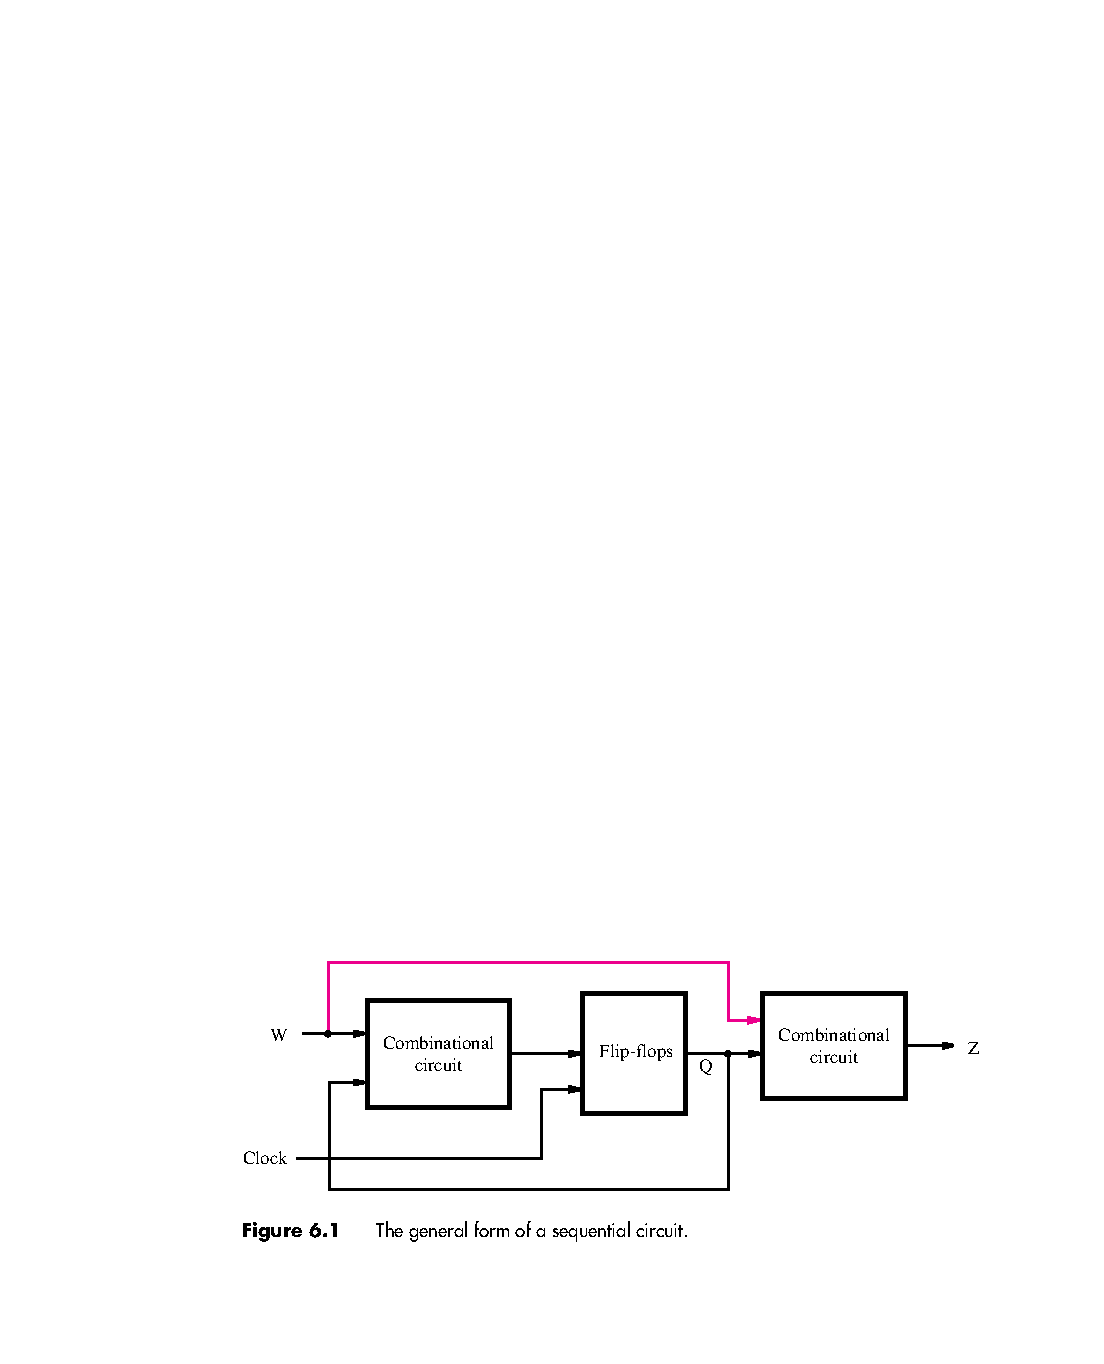
\includegraphics[width=\textwidth]{VerilogFig6_1} \\
    Edward Moore e George Mealy (1950s)
\end{frame}
% Síncronos = Clock

\begin{frame}{Circuitos Sequenciais Síncronos} 
    Considere uma aplicação para controlar a velocidade de um veículo. Um sensor \textit{w} indica quando ele está excedendo a velocidade desejada. Se isso ocorrer durante duas ou mais medidas consecutivas, um sinal \textit{z} deve ser acionado para reduzir sua velocidade. Estas são as especificações:
    \begin{enumerate}
        \item O circuito tem uma entrada, \textit{w}, e uma saída, \textit{z};
        \item Todas as mudanças no circuito ocorrem na borda positiva de \textit{clock}; 
        \item A saída \textit{z} é igual a \textbf{1} se a entrada \textit{w} for \textbf{1} durante os dois ciclos consecutivos anteriores de \textit{clock}.
    \end{enumerate}
    \centering
    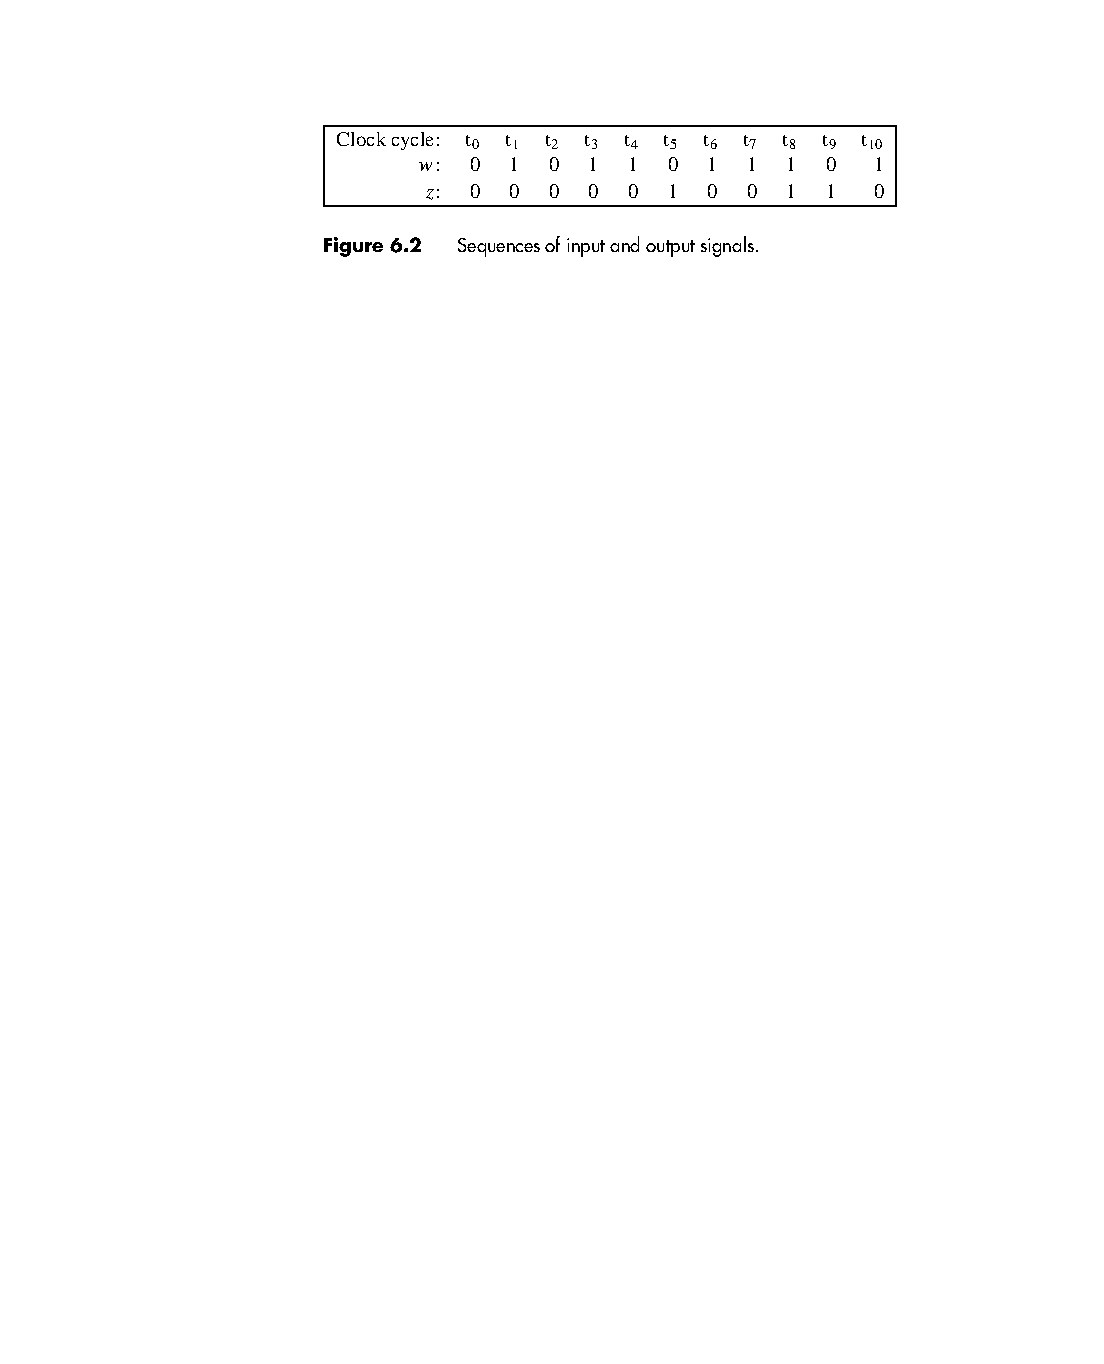
\includegraphics[width=.7\textwidth]{VerilogFig6_2} 
\end{frame}

\begin{frame}{Diagrama e Tabela de Estados} \centering
	\begin{columns}
        \column{0.3\textwidth}
        \vspace{3cm}
        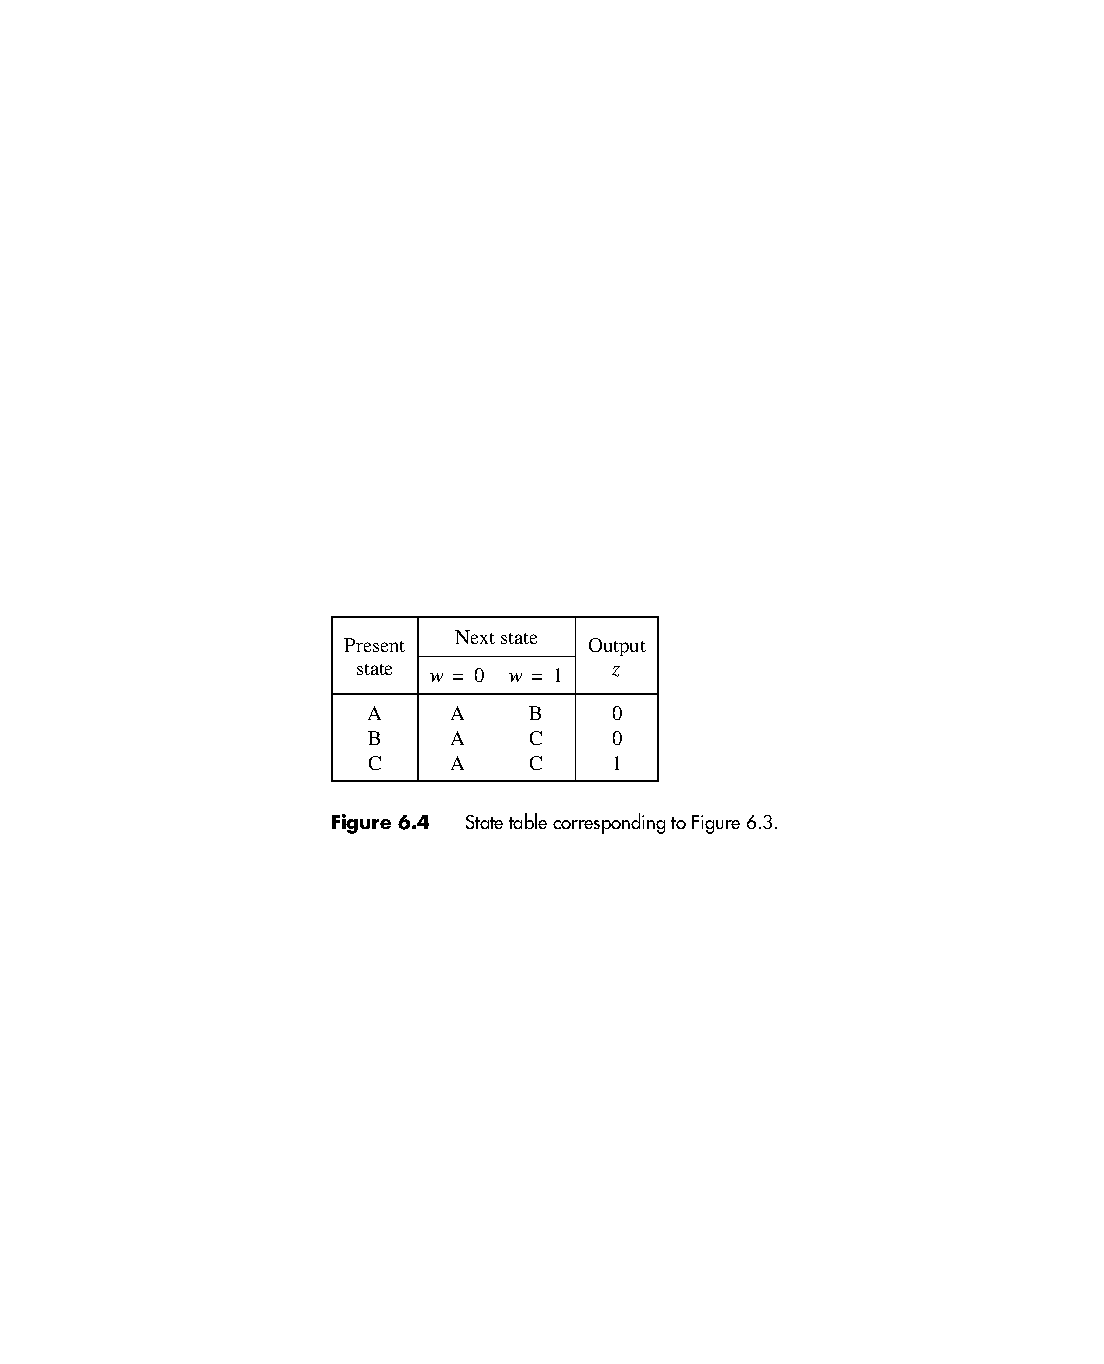
\includegraphics[width=2\textwidth,trim=0 1cm 0 0, clip]{VerilogFig6_4}
        \column{0.7\textwidth}
        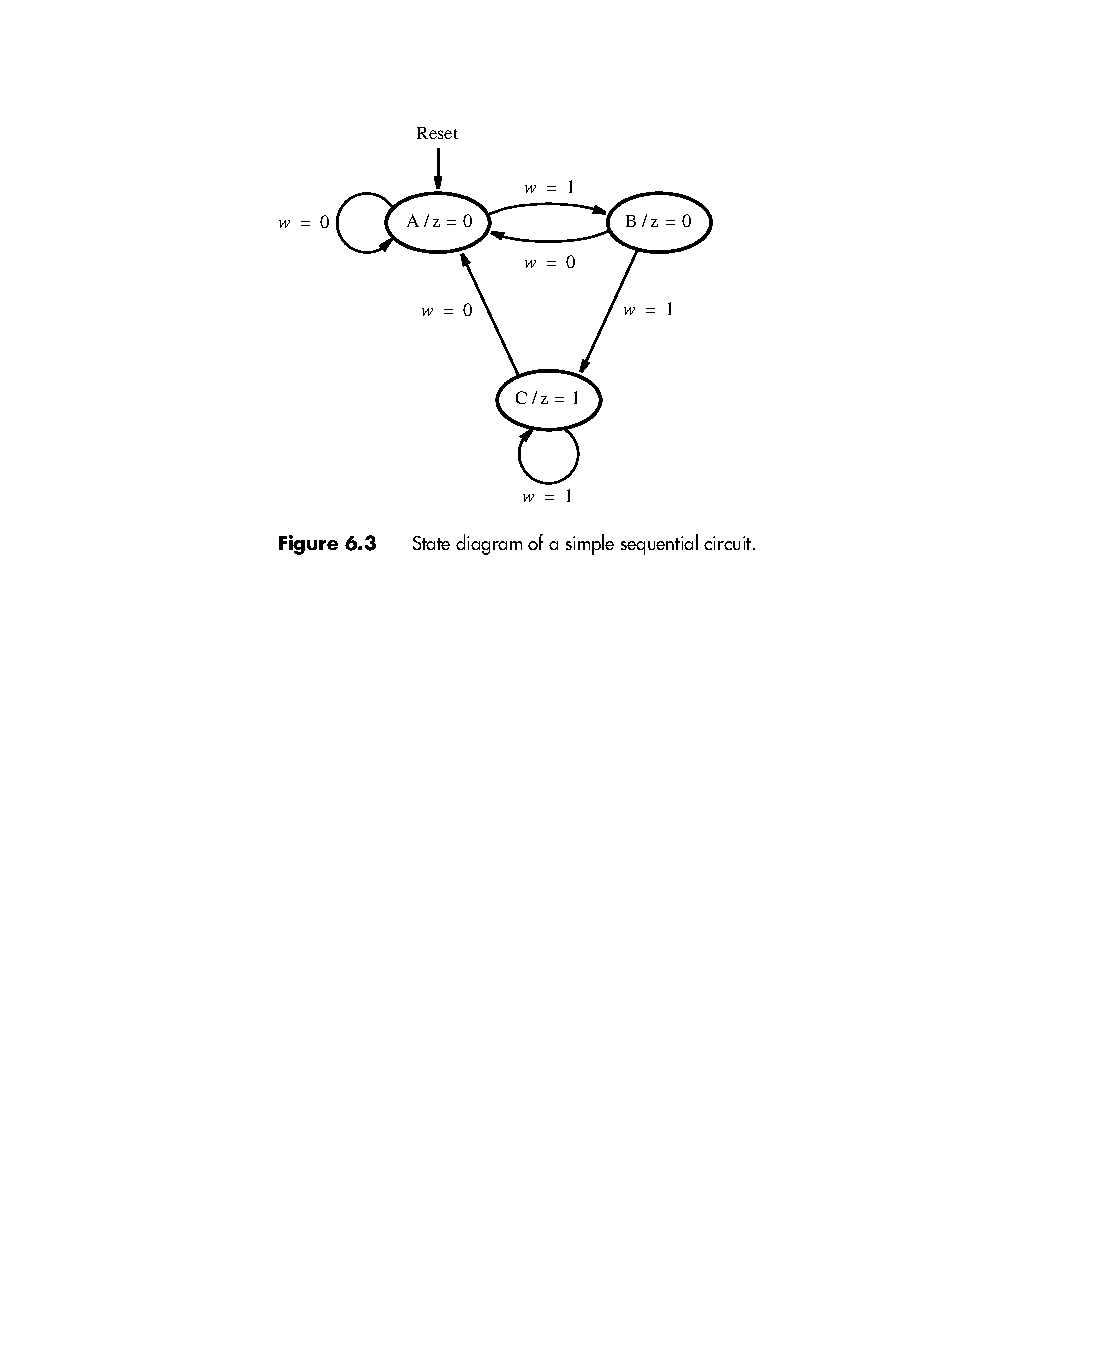
\includegraphics[width=\textwidth,trim=0 1cm 0 0, clip]{VerilogFig6_3}
	\end{columns}
\end{frame}

\begin{frame}{Forma geral do circuito} \centering
    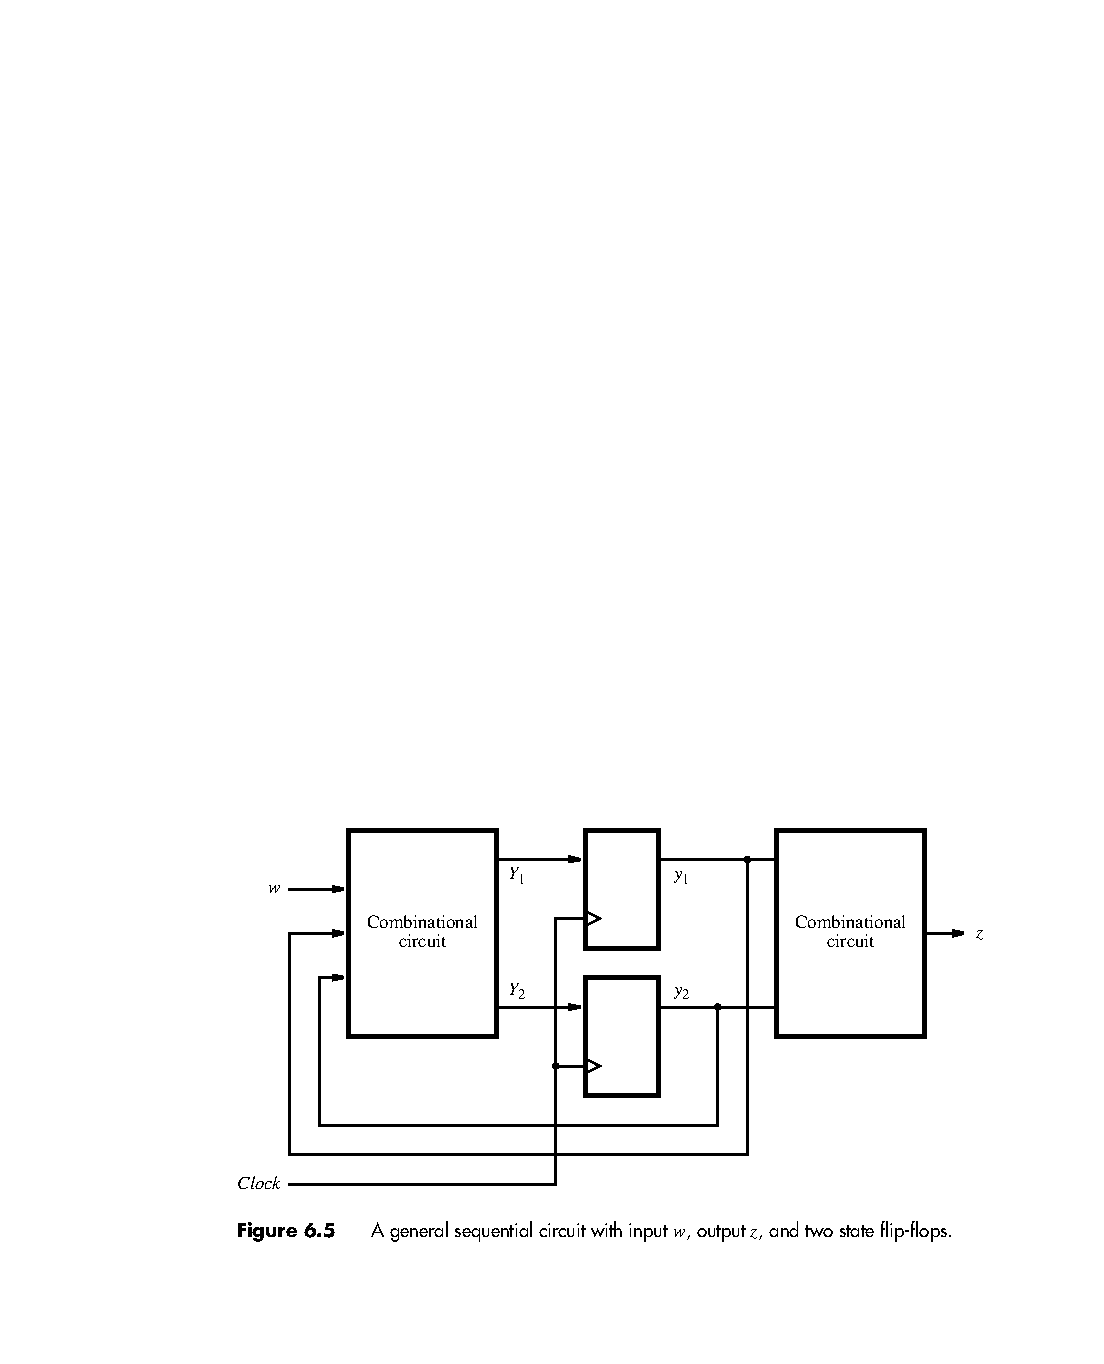
\includegraphics[width=.9\textwidth]{VerilogFig6_5} 
\end{frame}

\begin{frame}{Tabela de atribuição de estados} \centering
    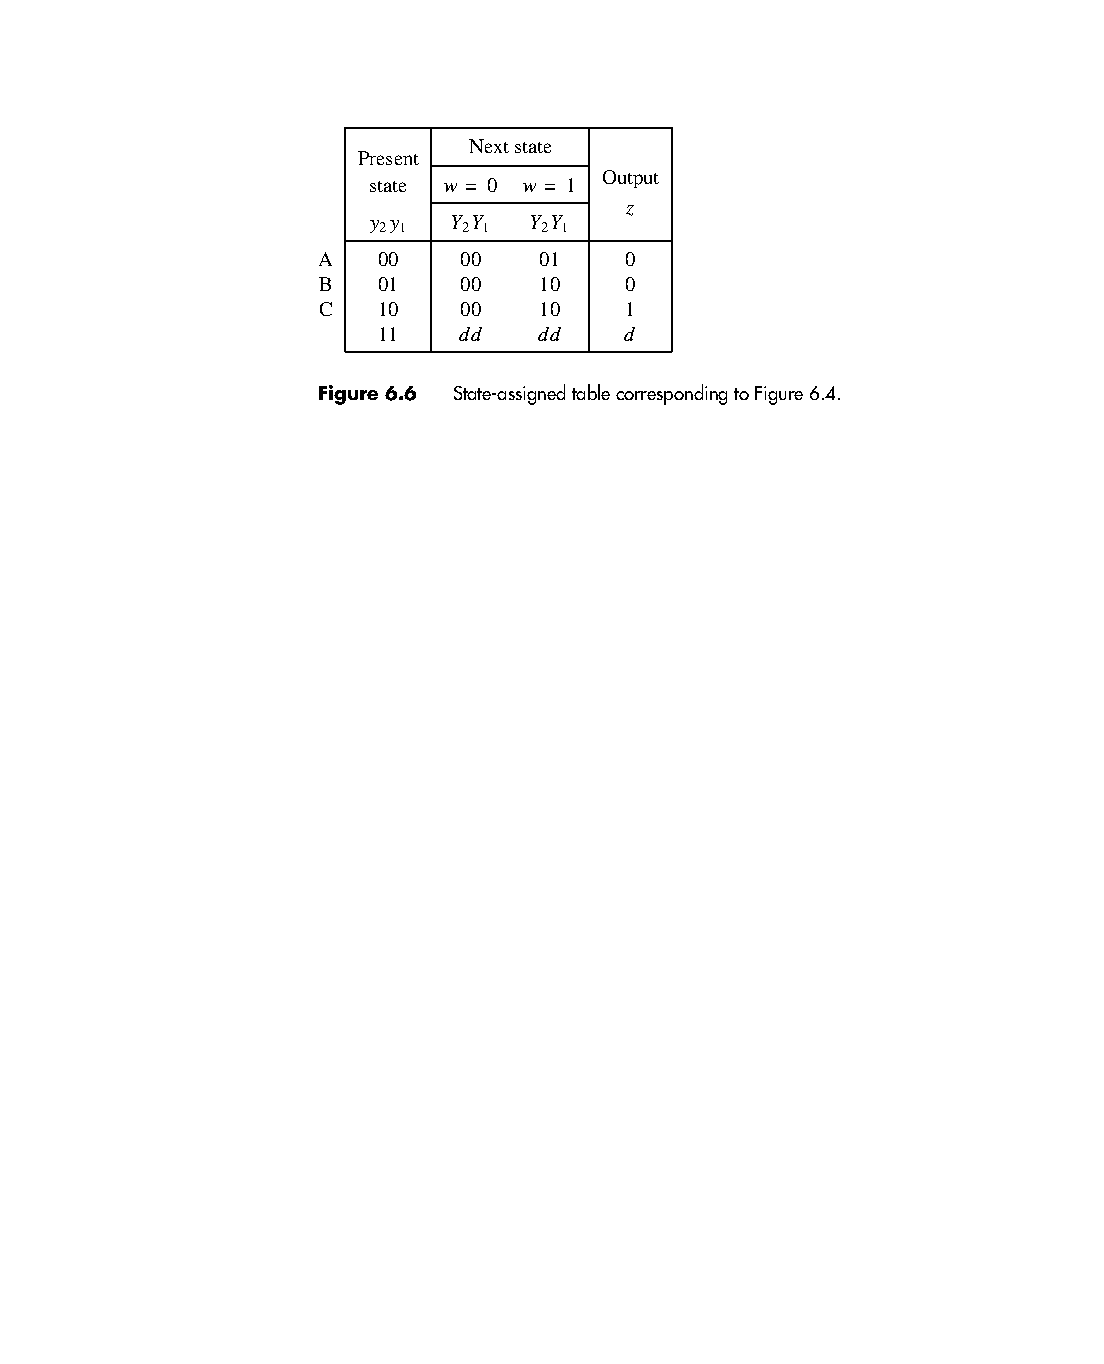
\includegraphics[width=.75\textwidth]{VerilogFig6_6} 
\end{frame}

\begin{frame}{Obtendo as expressões} \centering
    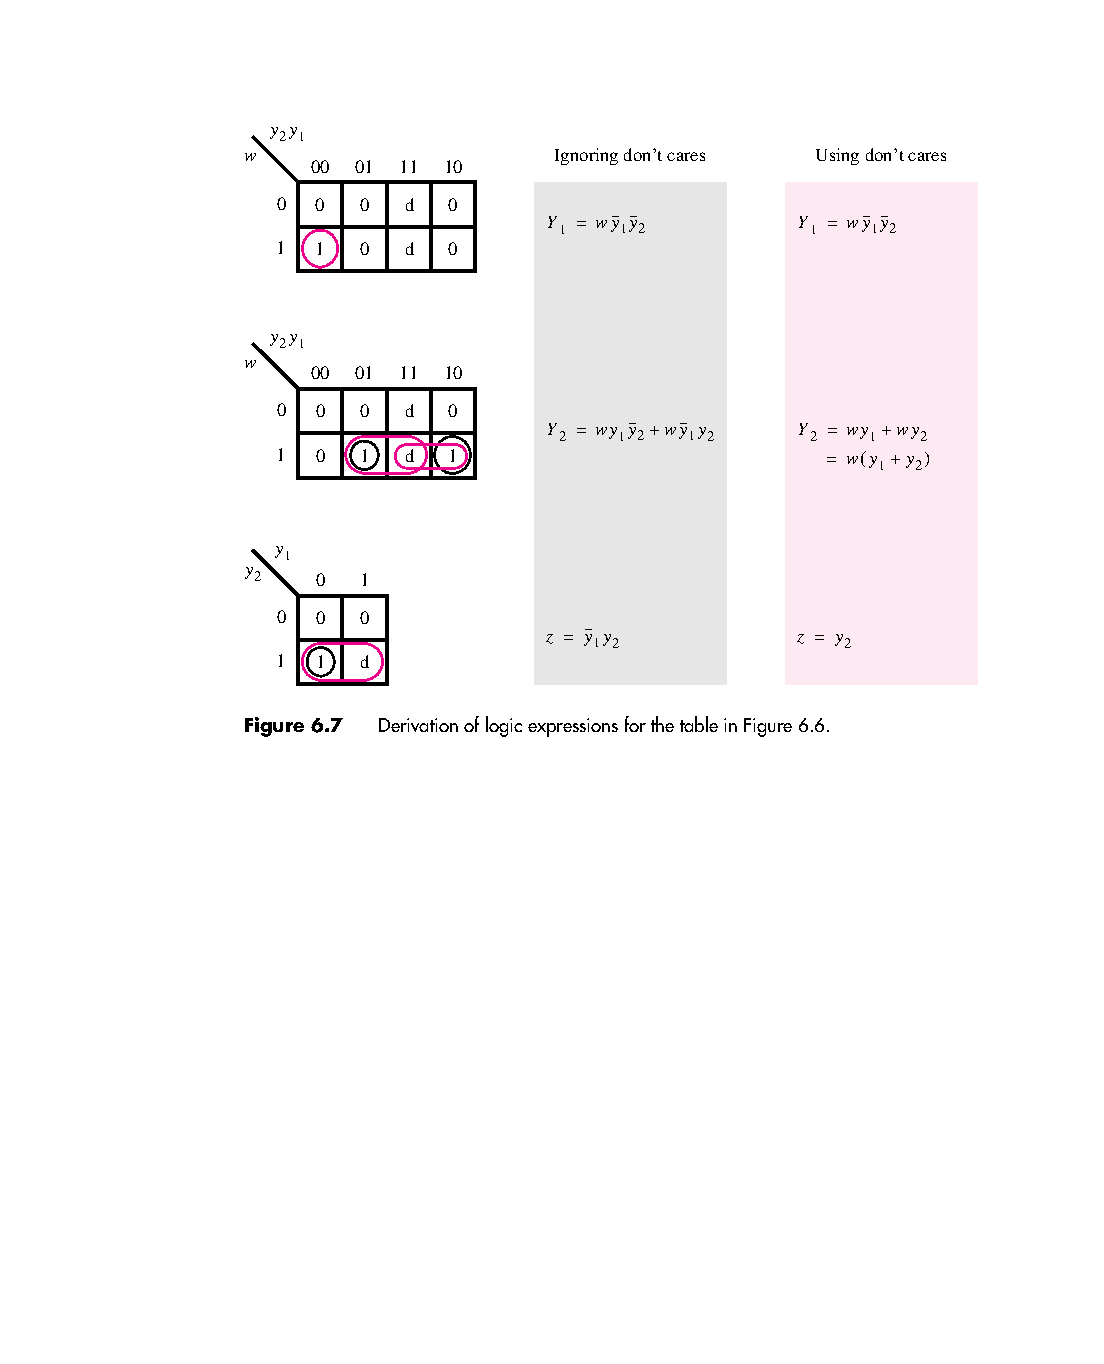
\includegraphics[height=.95\textheight]{VerilogFig6_7} 
\end{frame}

\begin{frame}{Circuito resultante} \centering
    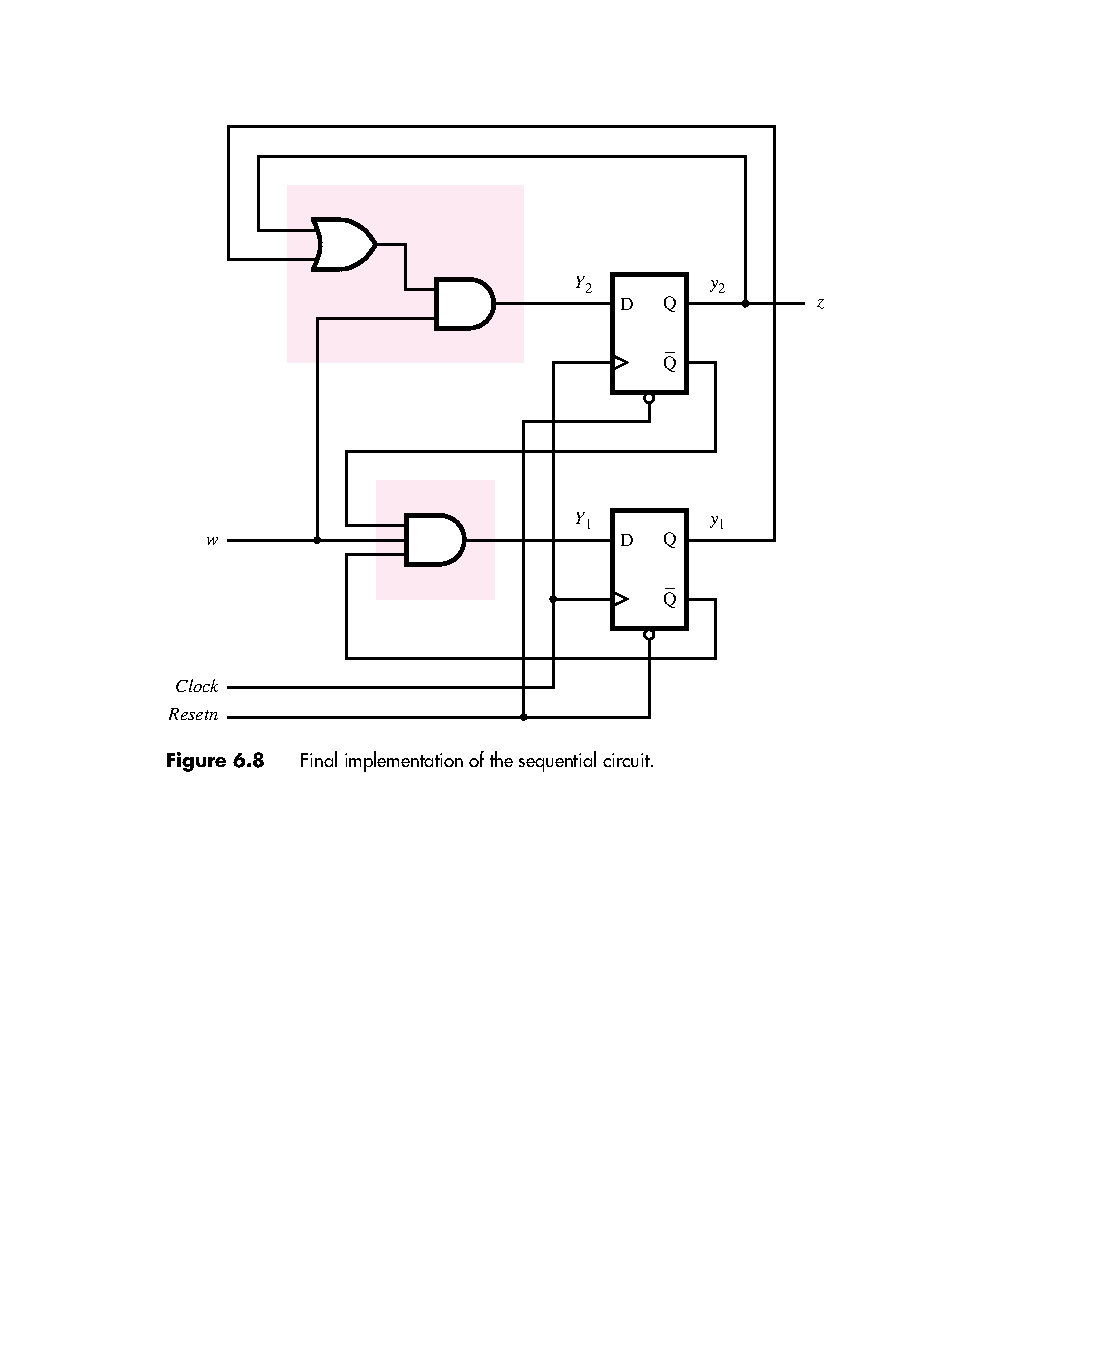
\includegraphics[height=.95\textheight]{VerilogFig6_8} 
\end{frame}

\begin{frame}{Simulação} \centering
    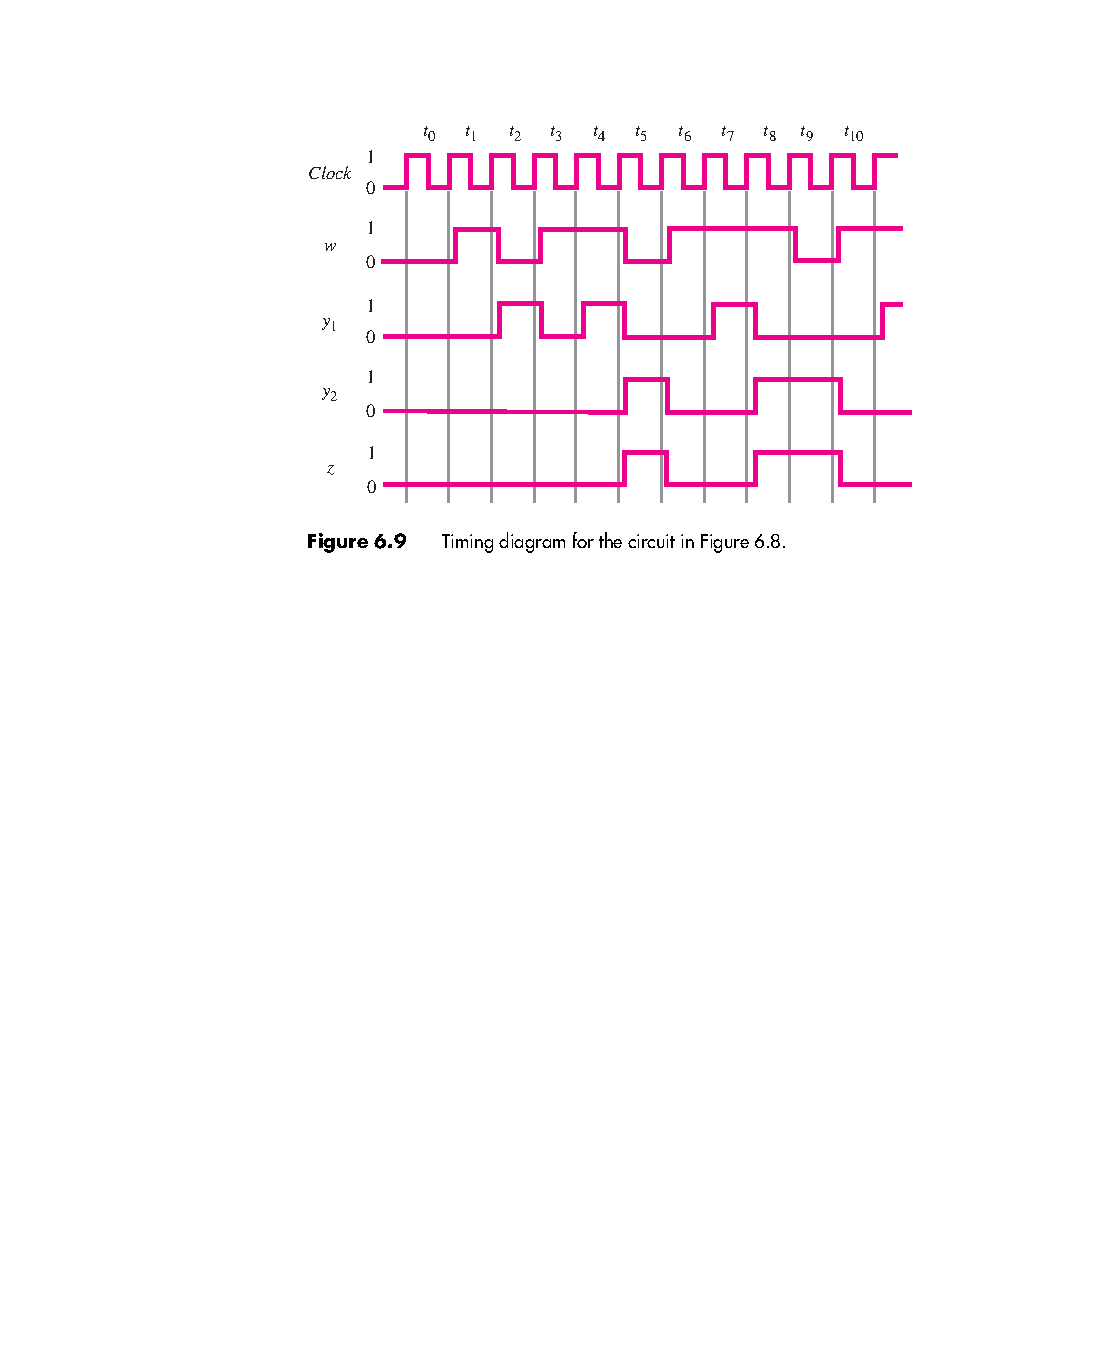
\includegraphics[height=.95\textheight]{VerilogFig6_9} 
\end{frame}

\begin{frame}{O problema da atribuição de estados} \centering
    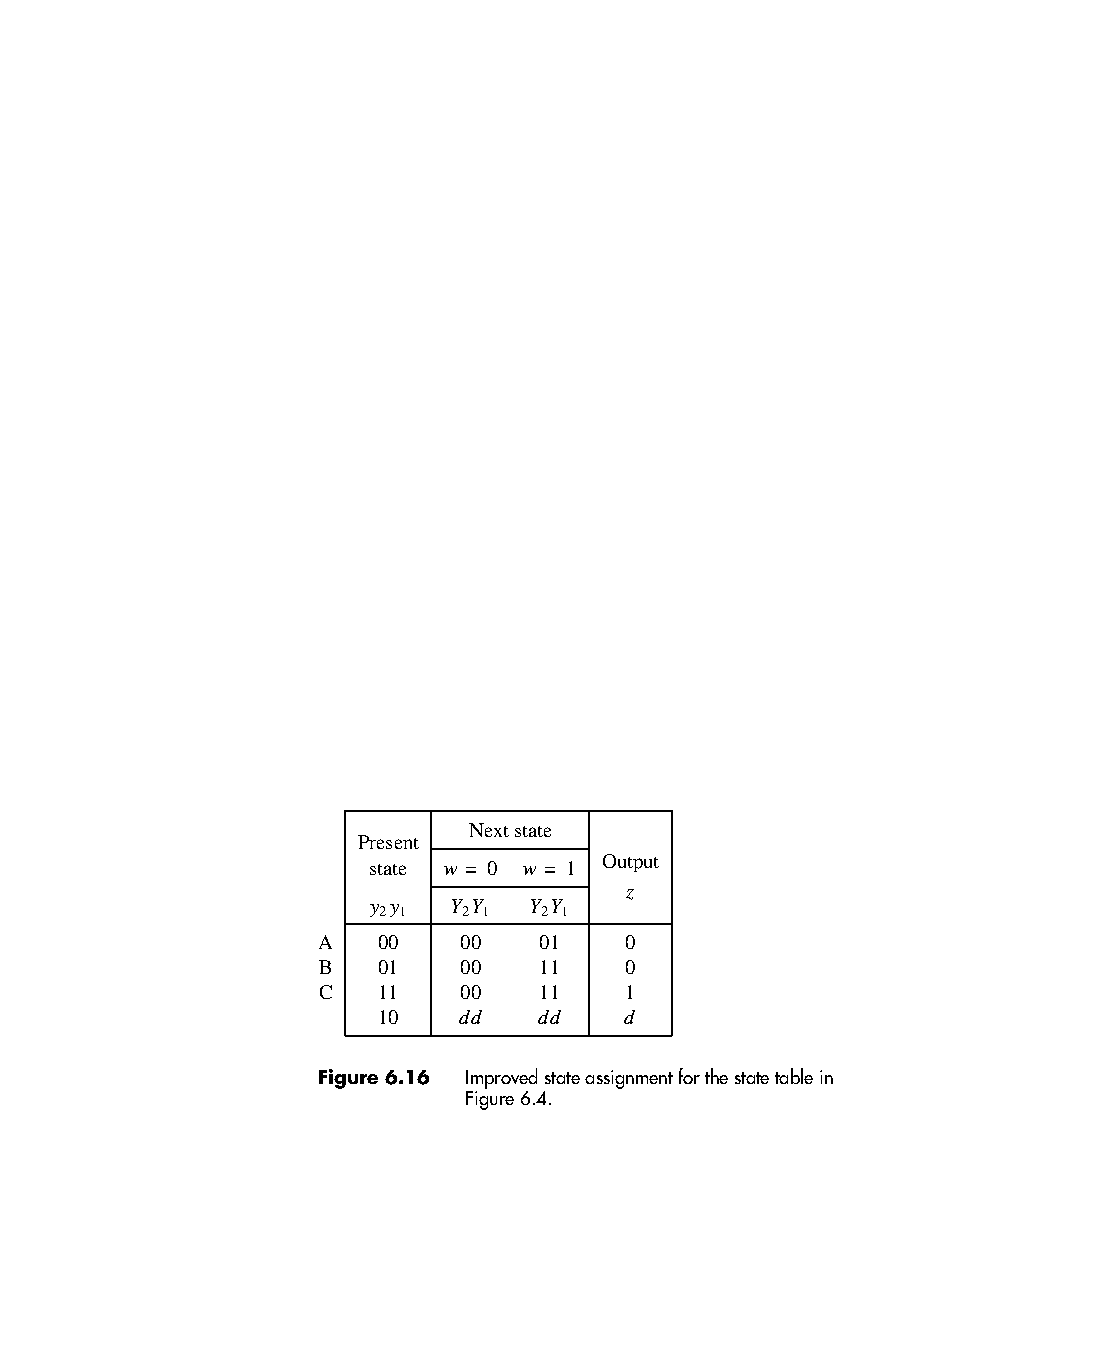
\includegraphics[height=.95\textheight]{VerilogFig6_16} 
\end{frame}

\begin{frame}{O problema da atribuição de estados} \centering
    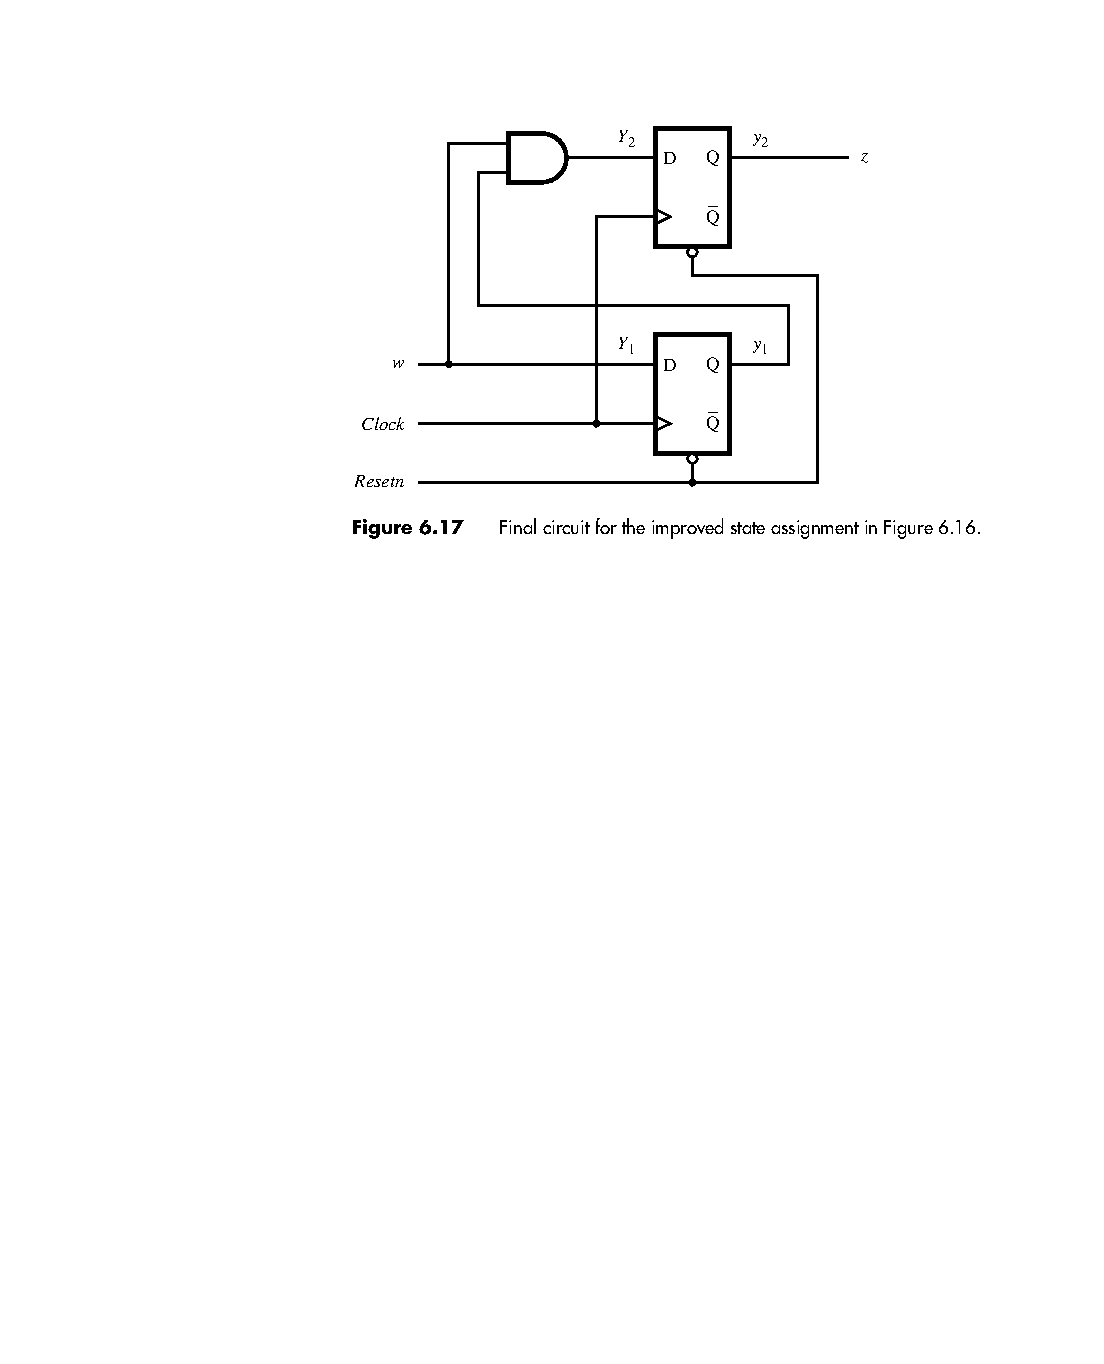
\includegraphics[height=.95\textheight]{VerilogFig6_17} 
\end{frame}


\begin{frame}{Resumo da metodologia} 
    Podemos resumir os passos para se obter um circuito sequencial síncrono da seguinte forma:
    \begin{enumerate}
        \item Obter a especificação do circuito desejado;
        \item Criar uma máquina de estados para o circuito. Partindo de um estado inicial, derivar os novos estados considerando todas as combinações de entradas possíveis; 
        \item Criar uma tabela de estados a partir da máquina de estados;
        \item Decidir o número de variáveis de estados necessário e atribuir valores a cada um deles; 
        \item Derivar as expressões de próximo estado e de saída; 
        \item Implementar os circuitos de acordo com as expressões. 
    \end{enumerate}
\end{frame}

\begin{frame}{Bibliografia} 
	\begin{itemize}
		\item \href{https://www.google.com.br/search?q=filetype\%3Apdf+Fundamentals+of+Digital+Logic+with+Verilog+Design+&oq=filetype\%3Apdf}{Brown, S. \& Vranesic, Z. - Fundamentals of Digital Logic with Verilog Design, 3rd Ed., Mc Graw Hill, 2009}
	\end{itemize}
\end{frame}

\begin{frame}
	\titlepage
\end{frame} 

\end{document}